\documentclass[12pt,a4paper]{article}

% --- Paquetes base (orden recomendado) ---
\usepackage[spanish,es-noshorthands]{babel} % <-- evita conflictos con TikZ
\usepackage[utf8]{inputenc}                 % Con Xe/LuaLaTeX puedes omitirla
\usepackage[T1]{fontenc}
\usepackage{lmodern}                        % Fuentes escalables
\usepackage{microtype}   



\usepackage{geometry}
\geometry{margin=2.5cm}
\usepackage{setspace}         % Interlineado 1,15
\usepackage{ragged2e}         % \justifying
\usepackage{fancyhdr}         % Encabezados/pies de página
\usepackage{hyperref}
\hypersetup{colorlinks=false}

% --- Tablas y columnas anchas ---
\usepackage{booktabs}
\usepackage{tabularx}
\usepackage{array}
\usepackage{makecell}
\usepackage[table]{xcolor}
\usepackage[section]{placeins} % fuerza a que los floats no crucen secciones


\newcolumntype{Y}{>{\RaggedRight\arraybackslash}X}

% --- Diagramas ---
\usepackage{tikz}
\usetikzlibrary{arrows.meta,positioning,babel,fit,shapes.symbols, calc}
\definecolor{becaccent}{HTML}{E84E36} % color acento (tú lo puedes cambiar)
\tikzset{
  block/.style={draw, rounded corners, align=center, minimum height=10mm, minimum width=32mm, inner sep=3pt},
}

% --- Imágenes y figuras
\usepackage{graphicx}     % incluir imágenes
\usepackage{caption}      % controlar estilo de leyendas (opcional)
\usepackage{float}        % para usar [H] (opcional)
\graphicspath{{figuras/}} % ruta por defecto para las imágenes (opcional)


% --- Estilo de página: número centrado abajo ---
\pagestyle{fancy}
\fancyhf{}
\cfoot{\thepage}
\renewcommand{\headrulewidth}{0pt}
\renewcommand{\footrulewidth}{0pt}

% --- Datos de portada ---
\newcommand{\Universidad}{Universidad Andrés Bello}
\newcommand{\Materia}{Tecnologías Disruptivas}
\newcommand{\NRC}{8090}
\newcommand{\Profesor}{Álvaro Sánchez Colmenares}
\newcommand{\NombreCaso}{Caso de estudio — Seguridad en Smart Cities}

% Integrantes ordenados por apellido + correos
\newcommand{\Integrantes}{%
  \begin{tabular}{@{}l}
    \textbf{Gabriel Cuevas}\\[-2pt]
    \texttt{\href{mailto:g.cuevasortzar@uandresbello.edu}{g.cuevasortzar@uandresbello.edu}}\\[6pt]
    \textbf{Alfredo Fuentes}\\[-2pt]
    \texttt{\href{mailto:a.fuentesnavarrete@uandresbello.edu}{a.fuentesnavarrete@uandresbello.edu}}\\[6pt]
    \textbf{Felipe Ochoa}\\[-2pt]
    \texttt{\href{mailto:f.ochoajohn@uandresbello.edu}{f.ochoajohn@uandresbello.edu}}\\[6pt]
    \textbf{Alonso Rodrigo Urra Villagra}\\[-2pt]
    \texttt{\href{mailto:a.urravillagra@uandresbello.edu}{a.urravillagra@uandresbello.edu}}\\[6pt]
    \textbf{Antonia Valdebenito}\\[-2pt]
    \texttt{\href{mailto:a.valdebenitofuentes@uandresbello.edu}{a.valdebenitofuentes@uandresbello.edu}}
  \end{tabular}
}

\newcommand{\Fecha}{\today}

\begin{document}

% --- Portada (sin número) ---
\pagenumbering{gobble}
\begin{titlepage}
  \centering
  \vspace*{1cm}
  {\Large \Universidad\par}
  \vspace{3cm}
  {\LARGE\bfseries \NombreCaso\par}
  \vspace{1.5cm}
  {\large \Materia\ (\textbf{NRC:} \NRC)\par}
  \vspace{0.4cm}
  {\large \textbf{Profesor a cargo:} \Profesor\par}
  \vspace{2.2cm}
  {\large \textbf{Integrantes}\par}
  \vspace{0.3cm}
  {\large \Integrantes\par}
  \vfill
  {\large \Fecha\par}
\end{titlepage}

% --- Cuerpo del informe ---
\clearpage
\pagenumbering{arabic}  % Numeración desde aquí
\setstretch{1.15}       % Interlineado 1,15
\justifying             % Texto justificado

\section*{Contexto del caso — Seguridad}

La ciudad ficticia \textit{Nueva Aurora} enfrenta un rápido crecimiento poblacional y se encuentra en un proceso de transformación hacia una \textit{Smart City}. En el eje de seguridad ciudadana, el desafío principal se manifiesta en el aumento de robos y en la baja integración de cámaras y sensores a nivel urbano, situación que limita la prevención, la reacción oportuna y la trazabilidad de incidentes.

Ante este contexto, la ciudad evalúa la adopción de tecnologías propias de las ciudades inteligentes —entre ellas, Internet de las Cosas (IoT), Inteligencia Artificial (IA), Big Data, \textit{blockchain}, 5G y soluciones energéticas asociadas— como base para articular un ecosistema de seguridad más proactivo, interoperable y basado en datos. Estas capacidades tecnológicas se consideran habilitadoras para la detección temprana de eventos, la coordinación táctica y la rendición de cuentas, con énfasis en el uso de IA en cámaras urbanas y el despliegue de sensores distribuidos.

\section{Definición del problema y alcance}

\subsection*{Problemas prioritarios}
\textbf{P1. Robos en espacio público y comercio de alta afluencia.} La ciudad evidencia un aumento sostenido de delitos contra la propiedad en zonas céntricas y nodos de transporte, afectando a peatones y locales comerciales.

\textbf{P2. Baja integración operativa de cámaras y sensores urbanos.} La infraestructura de videovigilancia y sensorización existe de forma fragmentada, sin interoperabilidad suficiente para detección temprana, trazabilidad ni coordinación de respuesta.

\subsection*{Causas principales}
\begin{itemize}
    \item \textit{Fragmentación tecnológica}: parques de cámaras heterogéneos, protocolos manuales y ausencia de estándares de intercambio de datos.
    \item \textit{Ceguera situacional}: escasa analítica de video en tiempo real y cobertura desigual de sensores (iluminación, aforos, botonería de alerta).
    \item \textit{Procesos reactivos}: tiempos de verificación largos por falta de correlación automática de eventos y evidencias.
    \item \textit{Limitaciones de infraestructura urbana}: iluminación deficiente y mobiliario que dificulta líneas de visión en puntos críticos.
\end{itemize}

\subsection*{Consecuencias}
\begin{itemize}
    \item \textit{Impacto ciudadano}: aumento de victimización y disminución de la percepción de seguridad.
    \item \textit{Ineficiencias operativas}: respuesta tardía y uso subóptimo de recursos de patrullaje y atención de emergencias.
    \item \textit{Baja trazabilidad}: dificultades para esclarecer hechos por falta de evidencia unificada y cadena de custodia digital.
\end{itemize}

\subsection*{Alcance del proyecto (fase piloto)}
\textbf{Área geográfica}: distrito céntrico de alta concurrencia (aprox. 3--4 km\textsuperscript{2}), que incluye eje comercial, dos estaciones de transporte masivo y tres intersecciones críticas.
\\
\textbf{Horizonte temporal}: 12 meses (3 meses diseño/instalación, 6 meses operación y ajuste, 3 meses evaluación).
\\
\textbf{Cobertura funcional}: integración de videovigilancia y sensores urbanos existentes, analítica de video en tiempo real para detección de eventos de riesgo, y tablero operativo para coordinación interinstitucional.
\\
\textbf{Procesos incluidos}: monitoreo preventivo, verificación de incidentes, despacho coordinado, preservación de evidencia digital y reportabilidad.

\subsection*{Fuera de alcance}
\begin{itemize}
    \item Reformas normativas o penales; reestructuración orgánica de fuerzas de orden.
    \item Vigilancia intrusiva en recintos privados o sin habilitación legal.
    \item Sustitución total de infraestructura existente fuera del polígono piloto.
\end{itemize}

\subsection*{Objetivos medibles (12 meses)}
\begin{itemize}
    \item Reducir en \(\geq 15\%\) los delitos contra la propiedad en el polígono piloto, respecto de la línea base.
    \item Disminuir en \(\geq 30\%\) el tiempo promedio de verificación y despacho ante eventos detectados.
    \item Alcanzar \(\geq 95\%\) de disponibilidad de la plataforma integrada (cámaras, sensores, analítica y tablero).
    \item Lograr que \(\geq 60\%\) de los incidentes relevantes sean \textit{detectados automáticamente} por analítica de video/sensores.
\end{itemize}

\subsection*{Restricciones y supuestos}
\begin{itemize}
    \item \textit{Legales y de privacidad}: tratamiento de datos personales sujeto a principios de finalidad, minimización y seguridad; difusión acotada de imágenes.
    \item \textit{Técnicas}: heterogeneidad de dispositivos; conectividad variable; necesidad de estándares abiertos (ONVIF, APIs seguras).
    \item \textit{Operativas}: coordinación interinstitucional y continuidad operativa 24/7 con personal capacitado.
\end{itemize}

\subsection*{Actores involucrados}
\begin{itemize}
    \item Municipio (gestión urbana y seguridad), centros de monitoreo y emergencia.
    \item Fuerzas de orden y equipos de respuesta (coordinación táctica y despacho).
    \item Comunidad y comercio local (canales de reporte y prevención situacional).
    \item Proveedores tecnológicos e integradores (infraestructura, software y soporte).
\end{itemize}

\subsection*{Riesgos y salvaguardas éticas}
\begin{itemize}
    \item \textit{Riesgos}: sesgos algorítmicos, vigilancia excesiva, ataques a la infraestructura, uso indebido de datos.
    \item \textit{Salvaguardas}: evaluación de impacto en privacidad, anonimización cuando corresponda, controles de acceso y auditoría, cifrado extremo a extremo, políticas de retención y uso proporcional de la información.
\end{itemize}


\newpage

\section{Mapa de problemas (Causa - Consecuencias)}
\subsection*{Problema 1: Robos en vía pública}
\textbf{Robos en vía pública} en zonas de alta influencia y nodos de transporte, con afectación directa a peatones y comercios. Vease la figura \ref{fig:mapa-problemas-seguridad}
\begin{figure}[htbp] % usa [H] si quieres fijarla exactamente aquí
  \centering
  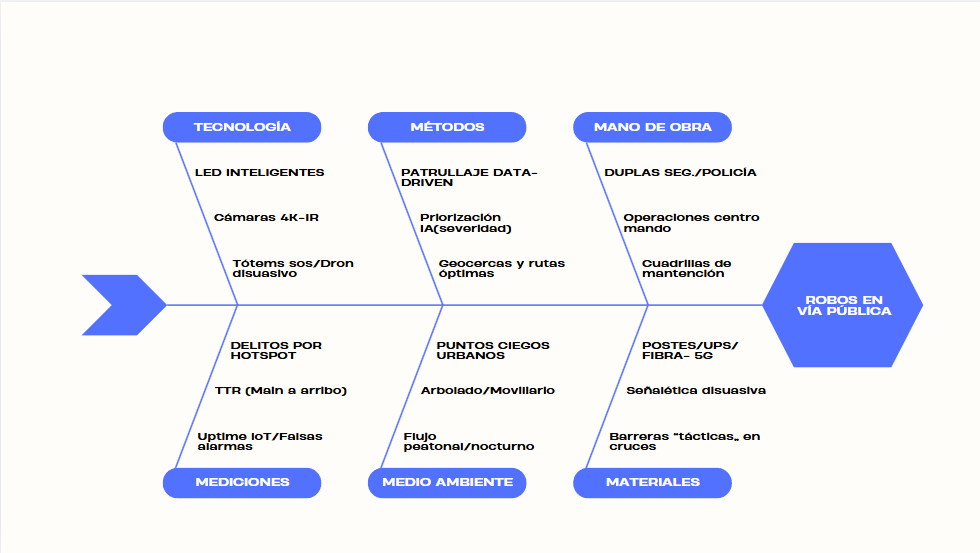
\includegraphics[width=\linewidth, keepaspectratio]{ishikawa_p1.png}
  \caption{Diagrama de Ishikawa del problema \textit{Robos en vía pública}.}
  \label{fig:mapa-problemas-seguridad}
\end{figure}

\subsection*{Causas inmediatas}
\begin{itemize}
    \item \textit{Fragmentación tecnológica}: Cámaras y sensores heterogéneos, con baja interoperabilidad y flujos manuales.
    \item \textit{Ceguera situacional}: Analítica de video limitada para detección temprana de eventos y cobertura desigual de sensorización.
    \item \textit{Procesos reactivos}: Verificación lenta por falta de correlación automática de alertas y evidencias.
    \item \textit{Infraestructura urbana subóptima}: Iluminación deficiente, mobiliario y arbolado que generan puntos ciegos.
\end{itemize}

\subsection*{Causa subyacentes}
\begin{itemize}
    \item \textit{Estándares y gobierno de datos insuficientes}: ausencia de APIs y protocolos abiertos para intercambio seguro.
    \item \textit{Capacidades operativas dispares}: roles, turnos y procedimientos no unificados entre vigilancia, monitoreo y despacho.
    \item \textit{Conectividad irregular}: tramos sin fibra/5G y respaldo eléctrico limitado que afectan la disponibilidad de equipos.
    \item \textit{Mantenimiento correctivo predominante}: fallas recurrentes y tiempos de reparación prolongados.
\end{itemize}

\subsection*{Consecuencias}
\begin{itemize}
    \item \textit{Impacto ciudadano}: Mayor victimización y disminución de la percepción de seguridad.
    \item \textit{Ineficiencias operativas}: Respuesta tardía y uso subóptimo de recursos de patrullaje y emergencia.
    \item \textit{Baja trazabilidad}: Dificultad para esclarecer hechos por carencia de evidencia integrada y cadena de custodia digital.
    \item \textit{Costos socioeconómicos}: Pérdidas para el comercio local y reducción de actividad en zonas críticas.
\end{itemize}

\subsection*{Relación causa–efecto (síntesis)}
\begin{table}[htbp]
\centering
\caption{Vinculación de causas con efectos del problema “Robos en vía pública”.}
\begin{tabular}{p{0.30\linewidth} p{0.36\linewidth} p{0.28\linewidth}}
\hline
\textbf{Categoría de causa} & \textbf{Evidencia/manifestación típica} & \textbf{Efecto principal} \\
\hline
Tecnología & Heterogeneidad de cámaras/sensores; sin correlación automática & Verificación lenta; baja detección temprana \\
Métodos & Patrullaje no dirigido por datos; rutas subóptimas & Cobertura reactiva; menor disuasión \\
Mano de obra & Roles/protocolos no unificados; capacitación desigual & Coordinación limitada en incidentes \\
Materiales & Iluminación insuficiente; señalética disuasiva escasa & Puntos ciegos y mayor oportunidad delictiva \\
Medio ambiente & Arbolado/mobiliario obstruyen; flujos peatonales desbalanceados & Zonas de riesgo persistentes \\
Mediciones & Falta de KPIs operativos; alto nivel de falsas alarmas & Mejora continua limitada \\
\hline
\end{tabular}
\end{table}

\subsection*{Indicadores asociados (línea base y metas)}
\begin{itemize}
    \item \textbf{Tasa de delitos contra la propiedad} (por 10\,000 hab.) en el polígono piloto: reducción relativa de \(\geq 15\%\) a 12 meses respecto de la línea base.
    \item \textbf{Tiempo medio de verificación y despacho (TTR)} desde la alerta hasta el envío de recurso: disminución de \(\geq 30\%\).
    \item \textbf{Disponibilidad de la plataforma integrada} (cámaras, sensores, analítica y tablero): \(\geq 95\%\).
    \item \textbf{Detección automática de incidentes relevantes} (analítica de video/sensores): \(\geq 60\%\) del total de incidentes registrados.
    \item \textbf{Tasa de falsas alarmas} (proporción sobre alertas totales): reducción a \(\leq 10\%\) mediante calibración y verificación.
\end{itemize}

\subsection*{Supuestos críticos}
\begin{itemize}
    \item Disponibilidad de conectividad (fibra/5G) y respaldo energético en puntos críticos.
    \item Acceso legal y seguro a datos para fines de prevención, reacción y trazabilidad, con políticas de minimización y retención.
    \item Coordinación interinstitucional efectiva para operación 24/7 y mantenimiento preventivo.
\end{itemize}


\subsection*{Problema 2: Baja integración operativa de cámaras y sensores}

\noindent La infraestructura de videovigilancia y sensorización urbana opera de forma fragmentada, con dispositivos heterogéneos y flujos de datos dispares. La ausencia de interoperabilidad y estandarización limita la detección temprana, la trazabilidad de incidentes y la coordinación de la respuesta.

\begin{figure}[htbp]
  \centering
  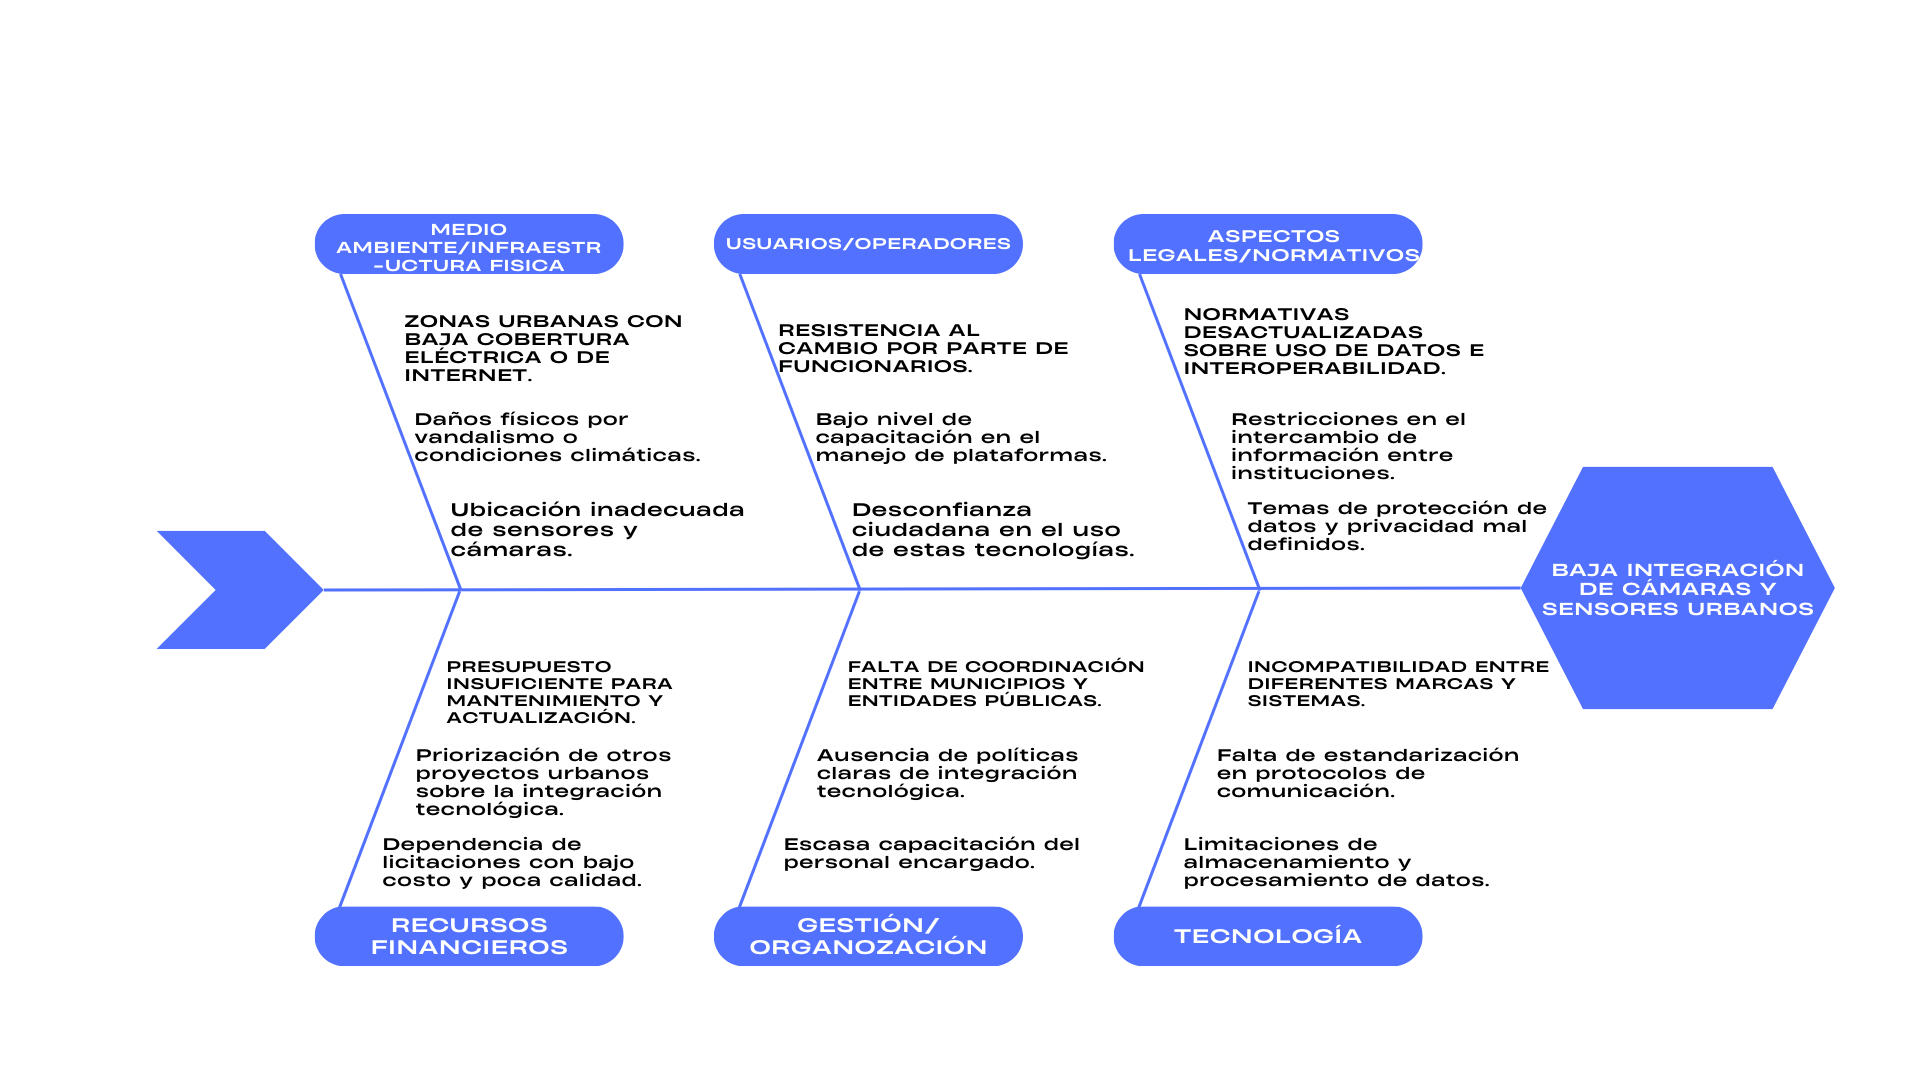
\includegraphics[width=\linewidth]{ishikawa_p2.png} % nombre actualizado
  \caption{Diagrama de Ishikawa — Problema 2: Baja integración operativa de cámaras y sensores.}
  \label{fig:ishikawa-p2}
\end{figure}

\subsection*{Causas inmediatas}
\begin{itemize}
    \item \textit{Fragmentación tecnológica}: dispositivos de distintos fabricantes sin adopción consistente de estándares abiertos (p.\,ej., ONVIF, APIs REST).
    \item \textit{Falta de integración}: inexistencia de un bus/middleware que unifique ingestión, normalización y distribución de eventos.
    \item \textit{Conectividad y energía irregulares}: enlaces sin redundancia y sin telemetría de salud en tiempo real.
    \item \textit{Procesos manuales}: verificación y correlación dependientes del operador, con alta variabilidad.
\end{itemize}

\subsection*{Causas subyacentes}
\begin{itemize}
    \item \textit{Gobierno de datos insuficiente}: políticas débiles de calidad, seguridad, retención y auditoría.
    \item \textit{Contratación por silos}: adquisiciones sin requisitos de interoperabilidad ni pruebas cruzadas.
    \item \textit{Observabilidad limitada}: carencia de métricas, logs y trazas end-to-end.
    \item \textit{Mantenimiento correctivo predominante}: inventario y versionamiento desactualizados.
\end{itemize}

\subsection*{Consecuencias}
\begin{itemize}
    \item \textit{Latencia operacional}: tiempos altos de detección y verificación con pérdida de ventanas de intervención.
    \item \textit{Baja trazabilidad}: dificultades probatorias por registros inconexos y cadena de custodia débil.
    \item \textit{Uso subóptimo de recursos}: despacho tardío y fatiga de operadores por falsas alarmas.
\end{itemize}

\subsection*{Relación causa–efecto (síntesis)}
\begin{table}[htbp]
\centering
\caption{Vinculación de causas con efectos del problema “Baja integración operativa”.}
\begin{tabular}{p{0.30\linewidth} p{0.36\linewidth} p{0.28\linewidth}}
\hline
\textbf{Categoría de causa} & \textbf{Evidencia/manifestación típica} & \textbf{Efecto principal} \\
\hline
Tecnología & Sistemas heterogéneos, sin perfiles ONVIF ni APIs alineadas & Imposibilidad de correlación; mayor latencia \\
Métodos & Verificación manual y scripts ad-hoc & Variabilidad operativa; tiempos de respuesta altos \\
Mano de obra & Capacitación dispar; dependencia del operador & Mayor tasa de error y falsas alarmas \\
Materiales & Falta de respaldo eléctrico y racks adecuados & Caídas de servicio; pérdida de datos \\
Medio ambiente & Interferencias/saturación en tramos inalámbricos & Pérdida de paquetes; jitter en video/eventos \\
Mediciones & Sin KPIs ni telemetría de salud & Mejora continua limitada; fallas no detectadas \\
\hline
\end{tabular}
\end{table}

\subsection*{Indicadores asociados (línea base y metas)}
\begin{itemize}
    \item \textbf{Cobertura integrada} (\% de cámaras/sensores gestionados desde la plataforma): meta \(\geq 85\%\).
    \item \textbf{Latencia de ingestión y correlación}: tiempo desde evento a alerta unificada; meta \(\leq 5\) s en críticos.
    \item \textbf{Incidentes con correlación automática}: proporción con video, georreferencia y recurso vinculado; meta \(\geq 70\%\).
    \item \textbf{Disponibilidad del servicio de integración}: meta \(\geq 99.5\%\) mensual.
    \item \textbf{Tasa de falsas alarmas}: meta \(\leq 10\%\).
\end{itemize}

\subsection*{Supuestos críticos}
\begin{itemize}
    \item Disponibilidad de enlaces confiables (fibra/5G) y respaldo energético en sitios críticos.
    \item Acceso legal a flujos de datos para prevención, reacción y trazabilidad, con principios de minimización y seguridad.
    \item Inventario técnico actualizado (modelos, firmware, topología) y adopción de estándares de interoperabilidad.
    \item Coordinación operativa 24/7 y mantenimiento preventivo programado.
\end{itemize}


\section{Ciudad referente}

\subsection*{1. Ciudad estudiada}
\textbf{Barcelona, España.} Ciudad europea pionera en infraestructura digital urbana, gobierno de datos y despliegues de sensorización y videovigilancia con analítica.

\subsection*{2. Tecnología concreta aplicada}
Plataforma urbana basada en estándares abiertos (p.~ej., \textit{Sentilo} para IoT) que integra:
\begin{itemize}
  \item Red de \textit{CCTV} con cámaras IP y perfiles ONVIF, enlazada a centros de control operativos.
  \item Sensores urbanos (iluminación telegestionada, aforo, acústica, calidad de aire, botonería de alerta).
  \item Analítica de video en tiempo real (detección de intrusión/merodeo, objetos abandonados, lectura de placas).
  \item Tableros operativos y geoespaciales para correlación evento--ubicación--recurso y despacho coordinado.
  \item Conectividad sobre fibra y redes móviles, con telemetría de salud para garantizar disponibilidad.
\end{itemize}

\subsection*{3. Resultados medibles reportados}
\begin{itemize}
  \item \textit{Operación}: incremento sostenido de disponibilidad de cámaras y reducción de tiempos de reparación al consolidar inventario y mantenimiento preventivo.
  \item \textit{Respuesta}: disminución de tiempos de verificación y despacho en zonas priorizadas gracias a la correlación automática (video + posición + recurso).
  \item \textit{Eficiencia energética}: ahorros significativos en alumbrado público por LED y telegestión (del orden de decenas de puntos porcentuales en áreas intervenidas).
  \item \textit{Investigación}: mayor proporción de incidentes con evidencia audiovisual útil y cadena de custodia digital.
\end{itemize}

\subsection*{4. Desafíos o riesgos observados}
\begin{itemize}
  \item Interoperabilidad y dependencia de proveedores: necesidad de exigir APIs abiertas y pruebas cruzadas.
  \item Continuidad operativa: vandalismo, energía y tramos con conectividad no redundada.
  \item Privacidad y ética: tratamiento proporcional de datos personales y mitigación de sesgos algorítmicos.
  \item Sostenibilidad: costos de mantenimiento/actualización y formación continua de operadores.
\end{itemize}

\subsection*{Adaptación al caso \textit{Nueva Aurora} (contexto latinoamericano)}
\begin{itemize}
  \item \textbf{Polígono piloto y línea base}: seleccionar zonas críticas y medir tasas de delitos, TTR y falsas alarmas previas a la intervención.
  \item \textbf{Interoperabilidad desde la compra}: requerir perfiles ONVIF, \textit{Sentilo}/APIs abiertas y pruebas de integración en licitaciones.
  \item \textbf{Middleware y tablero}: priorizar un bus de eventos y un tablero único con correlación video--evento--recurso.
  \item \textbf{Conectividad y energía}: fibra/5G con QoS y respaldo eléctrico en puntos críticos; telemetría de salud 24/7.
  \item \textbf{Gobierno de datos}: políticas de minimización, retención, auditoría y evaluación de impacto en privacidad.
  \item \textbf{Participación ciudadana}: botones de alerta, campañas de uso responsable y mecanismos de transparencia.
\end{itemize}


\end{document}
